\chapter{Testing and evaluation}

This chapter presents details of the implementations, experiments and evaluations for the Delta robot and testing system in previous chapter. Section 1 describes the experimental environment, which include hardware and supporting hardware. Subsequently, section 2 presents all the experiments along with evaluation and assessment.

\section{Experimental environment}
\subsection{Hardware configurations}
In accuracy and stability test, Delta robot is enough. The tests for the automated mobile app testing system are conducted with the hardware configurations as shown in table \ref{tab:hw}. We use 2 phones running 2 different \acrshort{os} versions with different screen size and resolution for testing the portability of the system.

\begin{table}[H]
	\centering
	\caption{Hardware configuration for testing process}	
	\label{tab:hw}
	\begin{tabularx}{0.65\textwidth}{ll}
		\toprule
		Phone 1 & ASUS Zenfone 5 \\
			  & Resolution 720 x 1280 pixels \\
			  & Screen 5'' 6.22 cm x 11.06 cm \\
			  & Android 5.0.1\\
		\midrule 
		Phone 2 & Sony XPeria L \\
			  & Resolution 480 x 850 pixels \\
			  & Screen 4.3'' 5.40 cm x 9.60 cm \\
			  & Android 4.2.2\\
		\midrule 
		Robot & Self-construct Delta Robot \\
			  & \begin{minipage}{0.5\linewidth}
				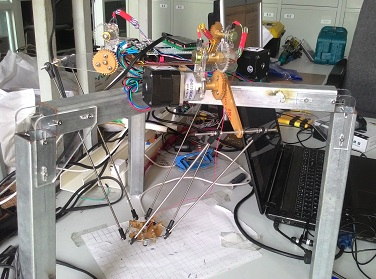
\includegraphics[width=0.8\linewidth]{Chapters/Fig/real_delta_robot.jpg}
				\end{minipage} \\
		\midrule 
		Computer & Windows PC \\
		\bottomrule
	\end{tabularx}
\end{table}

\subsection{Software}

In the test for automated mobile app testing system, beside running testing application, we are required to have the following software installed on the computer.

	\begin{itemize}
		\item[--] \textbf{Android platform tool}: command line tools for communicate with Android device.
		\item[--] \textbf{Droid@Screen}: application letting us capture Android screen to PC.
		\item[--] \textbf{Simple Click Test}: self-created tested application for Experiment 1.
		\item[--] \textbf{Clock ICS}: tested application for Experiment 2. This application can be downloaded on Google Play Store \footnote{Available at: \url{https://play.google.com/store/apps/details?id=com.moblynx.clockics}}
	\end{itemize}



\section{Testing and evaluation}

This section gives the details of all experiments that I have conducted to explore and evaluate accurate and stability of Delta robot, as well as it's feasibility in the real environment.

\subsection{Experiment 1: Test robot accuracy}
\subsubsection{Experiment's purpose}
Check the accuracy of the Delta Robot when moving to some points in workspace.
\subsubsection{Experimental setup}
Open test application, use control API to move end effector to a point.
\subsubsection{Experimental result and evaluations}
\begin{table}[H]
	\centering
	\caption{Experimental 1 result}	
	\label{tab:experiment_1}
	\begin{tabularx}{0.65\textwidth}{l|l}
		\toprule
		\textbf{Destination}	& \textbf{Real Coordinate} \\
		\midrule 
		$(0,0,-270)$			& $(0,0,-270)$ \\
		\midrule 
		\midrule 
		\bottomrule
	\end{tabularx}
\end{table}

%Robot hoạt động chính xác ở phần gần với trục Z, càng xa trục Z(x, y càng lớn) thì robot hoạt động càng kém chính xác hơn.

\subsection{Experiment 2: Test robot stability}
\subsubsection{Experiment's purpose}
Check the stability of the Delta Robot when running the test script repeatedly.
\subsubsection{Experimental setup}
Open test application, use control API to move end effector to a point and back repeatedly. Specifically, I move the end efector of Delta Robot from point $(-8, 0, -270)$ to $(-8, 0, -270)$ and back 10 times.

\subsubsection{Experimental result and evaluations}
\begin{table}[]
\centering
\caption{Experimental 2 result}
\label{tab:experiment_2}
\begin{tabular}{|l|l|l|}
\hline
\multirow{2}{*}{Times} & \multicolumn{2}{l|}{Value of potentiometer} \\ \cline{2-3} 
                       & (-80, 0, -270)        & (80, 0, -270)       \\ \hline
1                      & 526:288:490           & 526:507:289         \\ \hline
2                      & 524:286:490           & 524:505:290         \\ \hline
3                      & 524:286:491           & 524:506:291         \\ \hline
4                      & 526:288:490           & 525:507:289         \\ \hline
5                      & 525:288:490           & 524:505:289         \\ \hline
6                      & 526:287:491           & 524:505:290         \\ \hline
7                      & 526:288:490           & 526:506:291         \\ \hline
8                      & 527:288:489           & 524:505:290         \\ \hline
9                      & 526:288:489           & 524:507:290         \\ \hline
10                     & 523:288:490           & 526:505:292         \\ \hline
\end{tabular}
\end{table}
%Robot hoạt động ổn định dưới sai số cho phép của potentiometer(10%)

\subsection{Experiment 3: Simple Click test}
\subsubsection{Experiment's purpose}
Control the robot move and click on the screen, I can test the working accuracy of the robot when working in the testing system.
\subsubsection{Experimental setup}
Open Click test application.
\subsubsection{Experimental result and evaluations}
Begin test
	\begin{figure}[H]
		\centering
		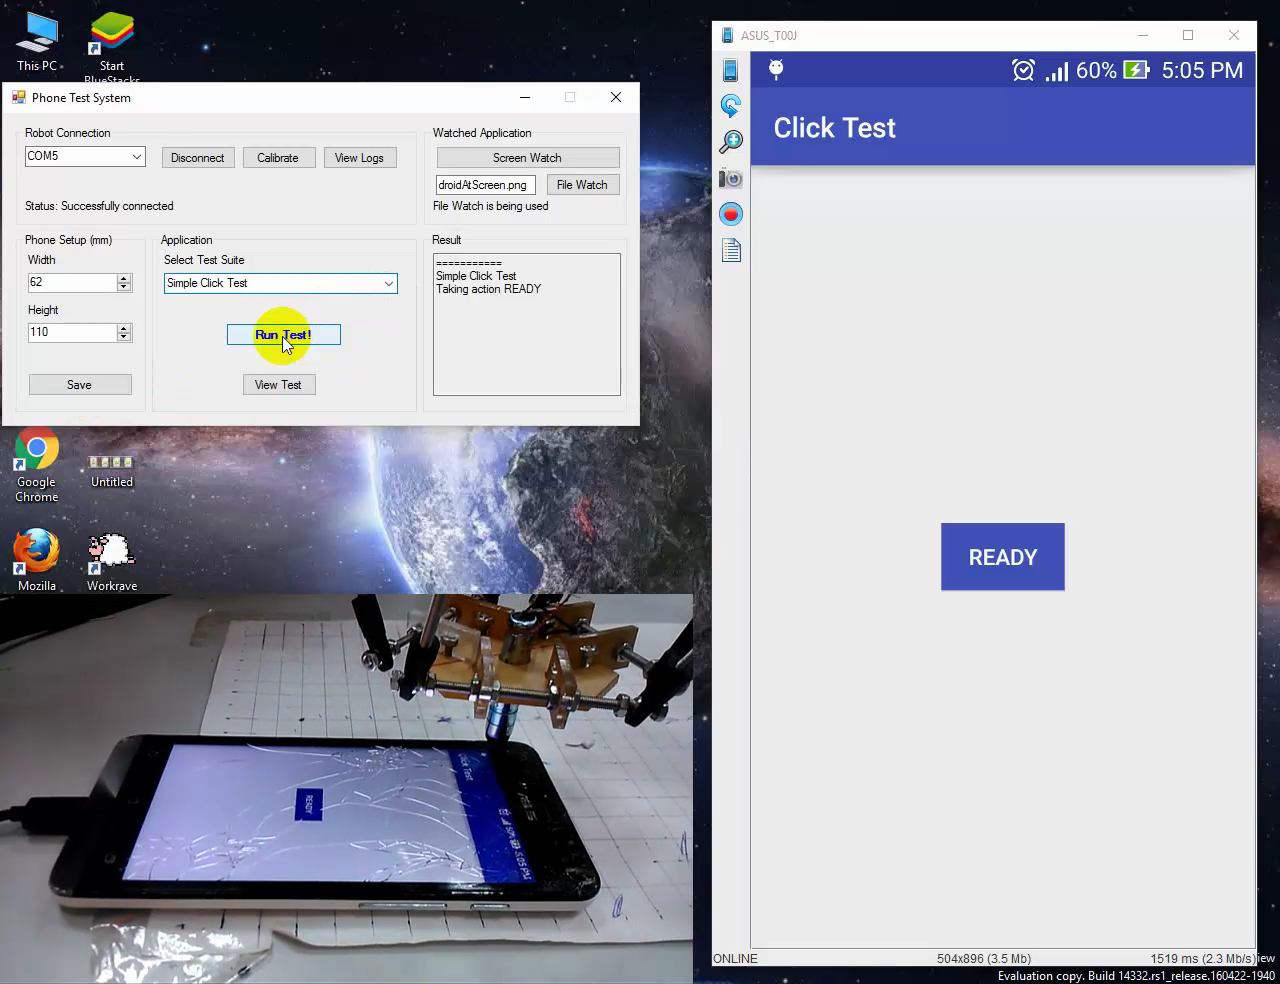
\includegraphics[width=\maxwidth{15cm}, keepaspectratio]{Chapters/Fig/click_start.png}
		\caption{Begin click test}
		\label{fig:click_start}
	\end{figure}

Final result
	\begin{figure}[H]
		\centering
		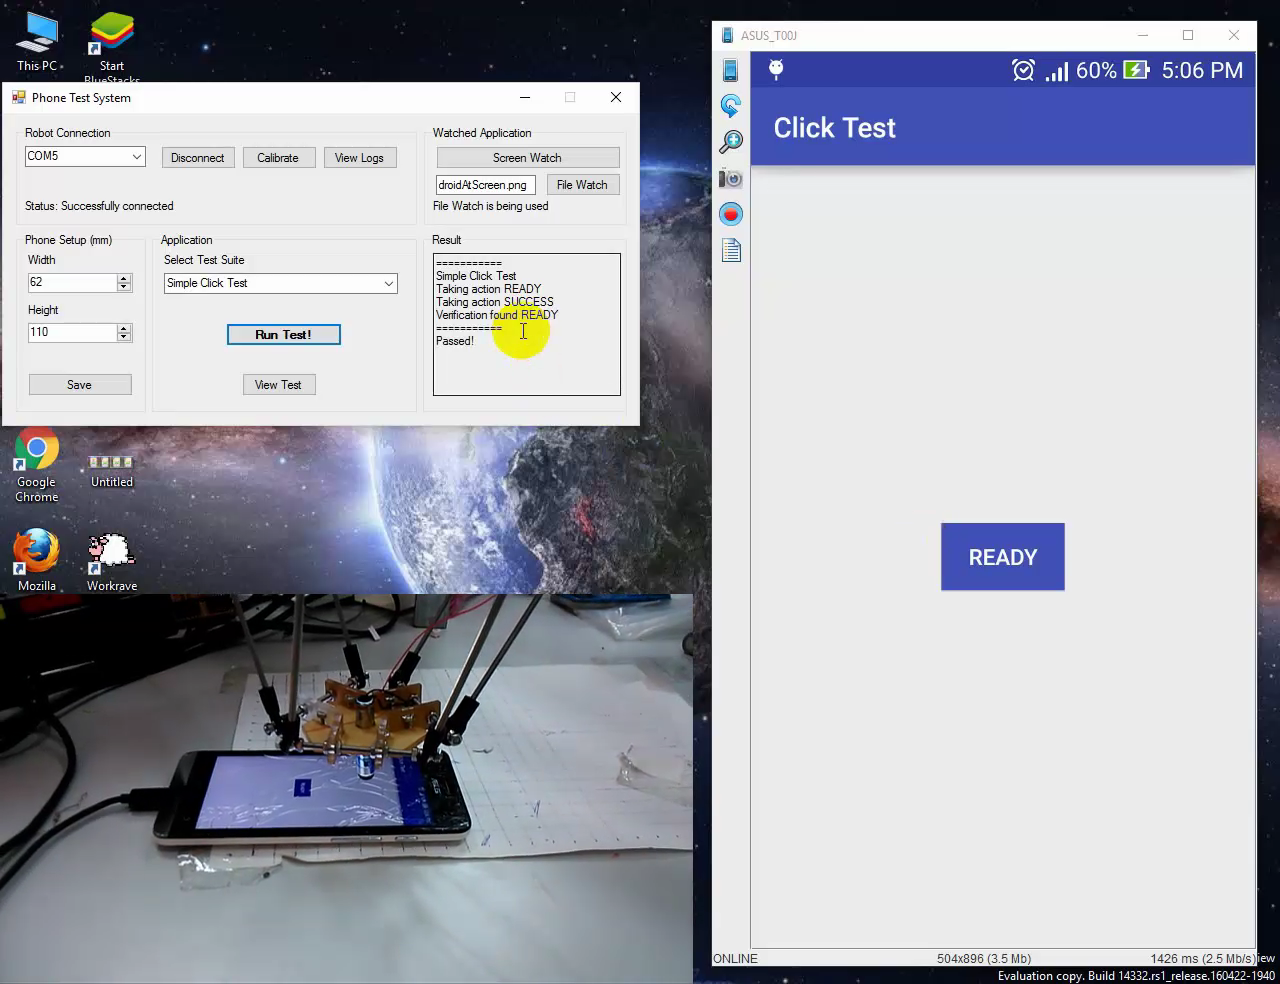
\includegraphics[width=\maxwidth{15cm}, keepaspectratio]{Chapters/Fig/click_final.png}
		\caption{Final click test}
		\label{fig:click_final}
	\end{figure}
\begin{table}[H]
	\centering
	\caption{Experiment 3: Test results statistic}	
	\label{tab:result_stat}
	\begin{tabular}{|lll|r|}
		\hline
		\textbf{Number of tests} & \textbf{Successful} & \textbf{Failed} & \textbf{Rate} \\
		\hline
		20 & 19 & 1 & 95$\%$\\
		\hline
	\end{tabular}
\end{table}
\subsection{Experiment 4: Set Alarm}
\subsubsection{Experiment's purpose}
Based on experiment control Delta robot select and setup alarm, I can test all the touch and swipe action
\subsubsection{Experimental setup}
Open Clock ICS application. Then open set alarm item.

\subsubsection{Experimental result and evaluations}
Begin test
	\begin{figure}[H]
		\centering
		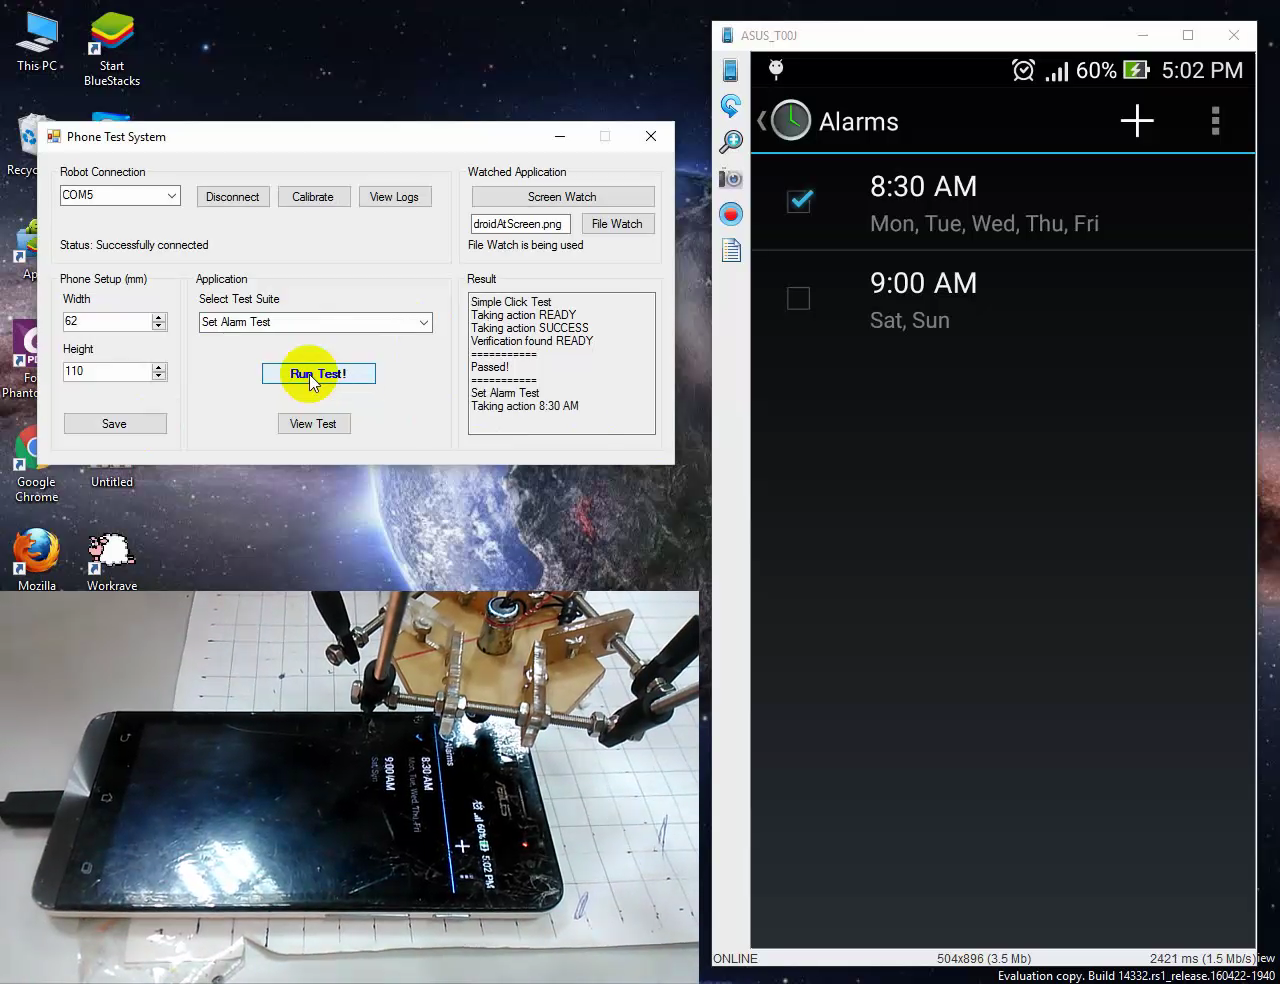
\includegraphics[width=\maxwidth{15cm}, keepaspectratio]{Chapters/Fig/alarm_start.png}
		\caption{begin alarm test}
		\label{fig:alarm_start}
	\end{figure}

Final result
	\begin{figure}[H]
		\centering
		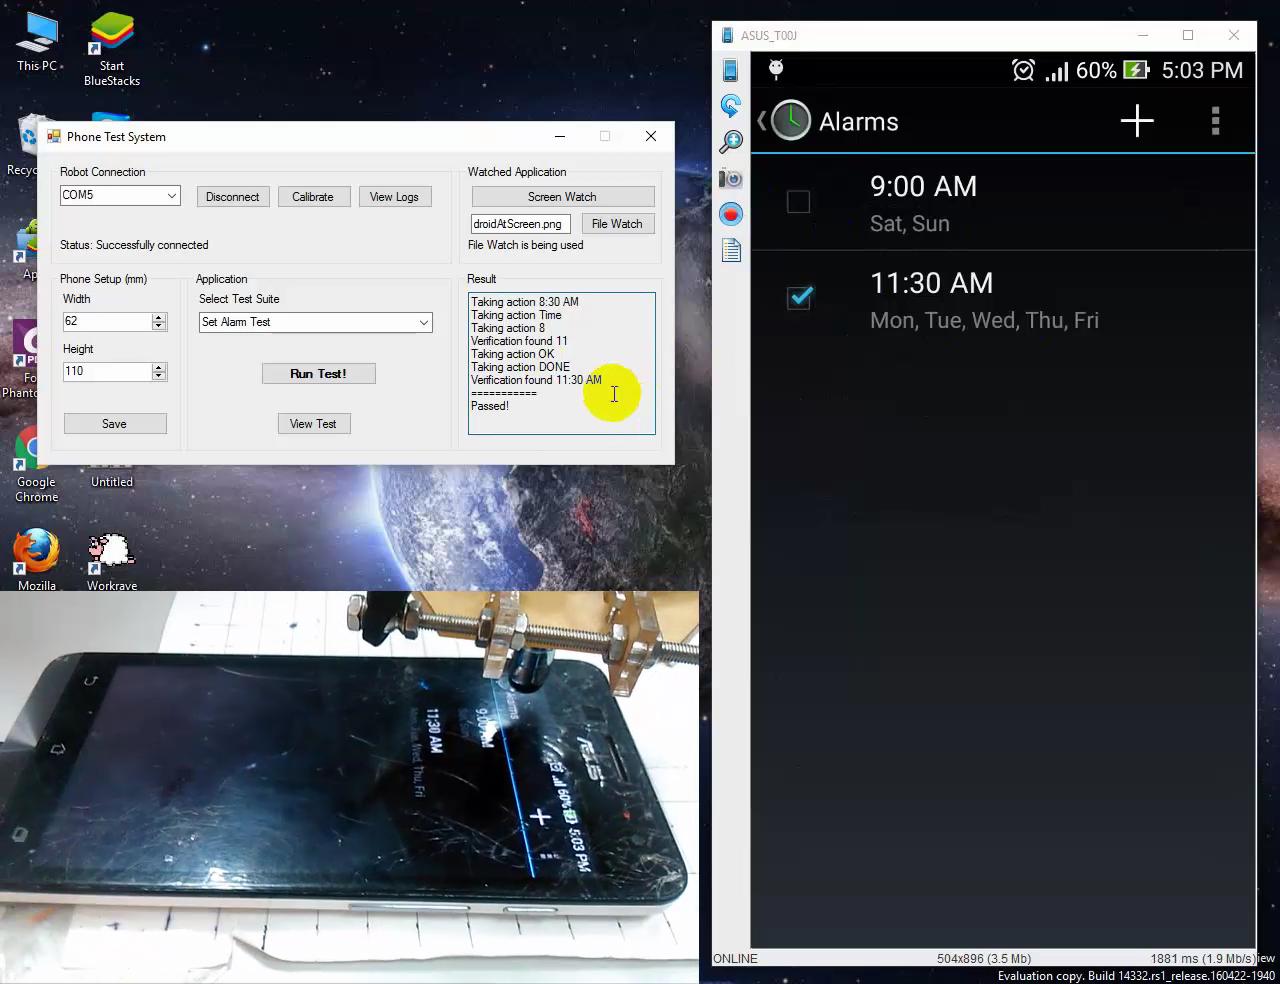
\includegraphics[width=\maxwidth{15cm}, keepaspectratio]{Chapters/Fig/alarm_final.png}
		\caption{final alarm test}
		\label{fig:alarm_final}
	\end{figure}
\begin{table}[H]
	\centering
	\caption{Experiment 4: Test results statistic}	
	\label{tab:result_stat}
	\begin{tabular}{|lll|r|}
		\hline
		\textbf{Number of tests} & \textbf{Successful} & \textbf{Failed} & \textbf{Rate} \\
		\hline
		10 & 6 & 4 & 60$\%$\\
		\hline
	\end{tabular}
\end{table}



